% Plantilla común para figuras redibujadas (fig-NN-desc.tex).
% Copiar entera y sustituir solo el cuerpo entre las marcas "cuerpo de la figura".
% Compila tal cual en Overleaf o con scripts/tikz2svg.sh.
%
% NO añadir la opción "tikz" a standalone: parte cada tikzpicture (y cada
% \chemfig) en una página distinta y el SVG solo tendría la primera.
\documentclass[border=4pt]{standalone}
\usepackage[T1]{fontenc}
\usepackage{lmodern}            % base vectorial: sin fuente vectorial el texto sale en Type 3 y dvisvgm lo pierde
\usepackage[scaled=0.95]{helvet}% sans-serif tipo Helvetica, como la interfaz de Obsidian
\renewcommand{\familydefault}{\sfdefault}
\usepackage{amsmath,amssymb}
\usepackage{sansmath}\sansmath  % fórmulas en sans, a juego con el texto
\usepackage[version=4]{mhchem}  % \ce{A + B -> C}
\usepackage{chemfig}            % estructuras y esquemas de reacción
\usepackage{tikz}
\usetikzlibrary{arrows.meta,positioning,calc,shapes.geometric,decorations.pathmorphing,decorations.markings}
\usepackage{pgfplots}           % gráficas (cinética, curvas de valoración...)
\pgfplotsset{compat=1.18}

% ---- Estilo Apuntes.md --------------------------------------------------
% Paleta semántica (la misma que el CSS de Obsidian). Principios inspirados en
% figures4papers (ChenLiu-1996, CC BY-NC 4.0): se adoptan ideas, no código.
\definecolor{apAzul}{HTML}{0F4D92}       % anotaciones, estructura (el azul del autor)
\definecolor{apAzulClaro}{HTML}{3775BA}
\definecolor{apRojo}{HTML}{B64342}       % curvas y datos principales, importante (el rojo del autor)
\definecolor{apRojoClaro}{HTML}{E9A6A1}
\definecolor{apVerde}{HTML}{3B7D3B}      % definiciones, "positivo"
\definecolor{apVerdeClaro}{HTML}{AADCA9}
\definecolor{apGris}{HTML}{767676}       % apoyo: rejillas, referencias, líneas punteadas
\definecolor{apGrisClaro}{HTML}{CFCECE}
\definecolor{apNegro}{HTML}{272727}      % ejes y texto neutro

\tikzset{
  % sin "color=" global: pisaría los \color{...} de chemfig (estructuras en rojo, etc.)
  every picture/.append style={line width=0.9pt, >={Stealth[length=2.4mm]}},
  curva/.style={apRojo, line width=1.6pt},                  % la curva o el dato que importa
  curva secundaria/.style={apAzulClaro, line width=1.3pt},
  referencia/.style={apGris, dotted, line width=1pt},       % líneas guía (p. ej. y = 0)
  anotacion/.style={apAzul, font=\normalsize},              % texto escrito a mano alrededor del dibujo
  flecha/.style={->, apAzul, line width=1pt},
  implica/.style={-{Implies}, double, double distance=2pt, line width=0.8pt},
  marca/.style={circle, fill=apAzul, draw=white, line width=0.6pt, inner sep=1.8pt},
  resalte/.style={apAzul, line width=1pt},                  % círculos/óvalos que rodean algo
}
\pgfplotsset{
  apuntes/.style={
    axis lines=left, axis line style={line width=1pt, apNegro, -{Stealth[length=2.4mm]}},
    tick style={apNegro, line width=0.8pt}, tick align=outside,
    label style={font=\normalsize}, tick label style={font=\normalsize},
    every axis plot/.append style={curva},
    clip=false,
  },
}
\setchemfig{atom sep=2em, bond style={line width=0.9pt}}
% -------------------------------------------------------------------------

\begin{document}
% --- cuerpo de la figura ---
% Genes -> (expresión génica) -> proteínas -> (plegamiento) -> funciones (pág. 10)
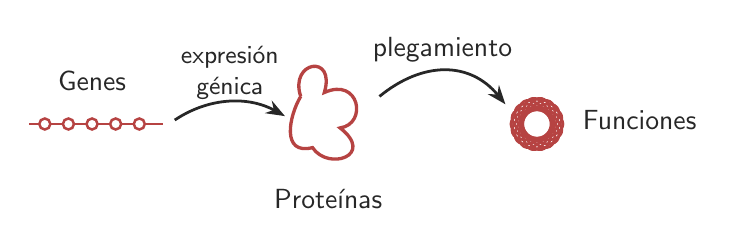
\begin{tikzpicture}[font=\normalsize]
  % genes: cadena de cuentas
  \node[apNegro] at (0.8,0.55) {Genes};
  \draw[apRojo, line width=1pt] (0,0) -- (1.7,0);
  \foreach \x in {0.2,0.5,...,1.6} \draw[apRojo, line width=0.9pt, fill=white] (\x,0) circle (0.07);
  % expresión génica
  \draw[->, apNegro, line width=1pt] (1.85,0.05) .. controls (2.3,0.35) and (2.8,0.35) .. (3.25,0.1);
  \node[apNegro, align=center, font=\small] at (2.55,0.65) {expresión\\génica};
  % proteína desplegada
  \draw[apRojo, line width=1.2pt] (3.45,0.35) .. controls (3.3,0.8) and (3.9,0.9) .. (3.75,0.4)
    .. controls (4.2,0.6) and (4.3,0.0) .. (3.95,-0.05) .. controls (4.4,-0.4) and (3.8,-0.6) .. (3.6,-0.3)
    .. controls (3.2,-0.4) and (3.3,0.1) .. (3.45,0.35);
  \node[apNegro] at (3.8,-0.95) {Proteínas};
  % plegamiento
  \draw[->, apNegro, line width=1pt] (4.45,0.35) .. controls (5.0,0.8) and (5.6,0.8) .. (6.05,0.25);
  \node[apNegro] at (5.25,0.95) {plegamiento};
  % proteína plegada (ovillo compacto)
  \foreach \a in {0,40,...,320} \draw[apRojo, line width=1pt, rotate around={\a:(6.45,0.0)}] (6.45,0.0) ellipse (0.33 and 0.18);
  \node[apNegro, anchor=west] at (6.9,0.05) {Funciones};
\end{tikzpicture}
% ---------------------------
\end{document}
